\section{TP2 : Transmission non bruitée analogique}
\sectionmark{TP2 : Transmission non bruitée analogique}

\subsection{Introduction étape 2}
Dans la continuité de l'étape 1, nous étudierons le comportement du système de transmission en tenant compte de la nature analogique du canal de transmission. Nous aborderons ainsi les différents types de codages analogiques implémentés.

\begin{figure}[H]
    \centering
    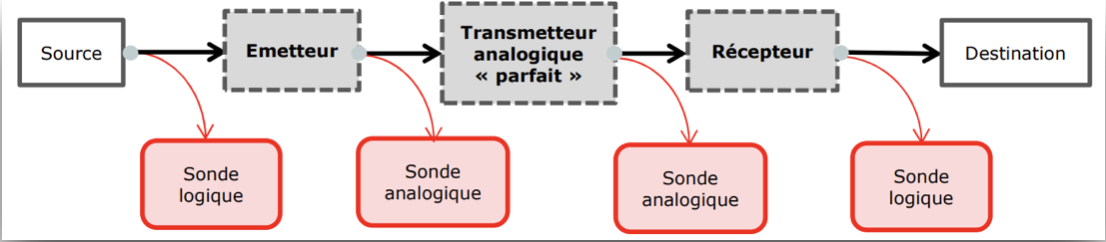
\includegraphics[width=0.7\textwidth]{img/etape2_chaine_transmission.png}
    \caption{Chaîne de transmission}
    \label{fig:teb1}
\end{figure}

\subsection{Objectifs}
Pour cette deuxième étape, nous maintenons la capacité d'envoyer un message binaire, mais avec un transmetteur analogique \textit{parfait} qui garantit un TEB de 0. Les nouveautés liées au transmetteur analogique incluent le choix de la forme d'onde et la spécification du nombre d'échantillons par bit ainsi que les amplitudes min et max.

\subsection{Paramètres du logiciel}
Le paramètre \texttt{form f} permet de spécifier la forme d'onde pour la transmission analogique. Les options disponibles sont :

\begin{enumerate}
    \item \textbf{NRZ} : Forme d'onde rectangulaire.
    \item \textbf{NRZT} : Forme d'onde trapézoïdale (temps de montée et de descente, respectivement à 1/3 du temps bit).
    \item \textbf{RZ} : Forme d'onde impulsionnelle (amplitude minimale sur le premier et dernier tiers du temps bit, impulsionnelle sur le tiers central avec un maximum au milieu du temps bit égal à l'amplitude maximale).
\end{enumerate}

Par défaut, le simulateur utilise la forme d'onde RZ pour le signal analogique.

Le paramètre \texttt{nbEch ne} permet de spécifier le nombre d'échantillons par bit dans la transmission analogique. Il doit être une valeur entière positive. Par défaut, le simulateur utilise 30 échantillons par bit.

Le paramètre \texttt{ampl min max} spécifie l'amplitude minimale et maximale du signal analogique. Ils doivent être des valeurs flottantes, avec min < max. Par défaut, le simulateur utilise 0.0f comme valeur minimale et 1.0f comme valeur maximale.

\subsection{Réallisation}
Pour la gestion de projet, nous avons opté pour l'outil Taiga. Cet outil nous permet de définir les tâches attribuées à chaque membre de l'équipe, d'organiser la planification et de prioriser lesdites tâches. En ce qui concerne le développement logiciel, nous utilisons un dépôt Git sur GitHub. Cette approche permet à tous les membres de l'équipe d'accéder facilement au code et assure une traçabilité de toutes les versions.

\subsection{Émetteur analogique}
Dans notre contexte de chaîne de transmission analogique, nous avons établit que nous devions faire la chaîne de transmission par l’adjonction de deux étages (logique → analogique et analogique → logique). Pour ce faire, nous allons tout d’abord nous intéresser à l’émission de notre signal. 

Dans notre code, les classes \textbf{Emetteur} et \textbf{Recepteur} doivent être modifiées pour gérer l’emission analogique. Notamment la prise en charge de trois formes d’ondes: NRZ, NRZT et RZ. Chaque type d’onde aura une méthode dédiée qui nous permettra de réaliser son traitement.

\subsubsection{Émission analogique NRZ}
Le codage NRZ (Non Return to Zero) permet la transmission d’un signal via un système d’échelonnage. Il représente une des manière les plus simple de transmission car il n’y a pas de niveau intermédiaire, mais seulement deux états binaire 0 et 1 :

\begin{itemize}
    \item Bit à 1 en entrée : le flottant (correspondant à la valeur du signal) prend comme valeur l’amplitude maximal $A_{max}$
    \item Bit à 0 en entrée : le flottant (correspondant à la valeur du signal) prend comme valeur l’amplitude minimal $A_{min}$
\end{itemize}

\begin{figure}[H]
    \centering
    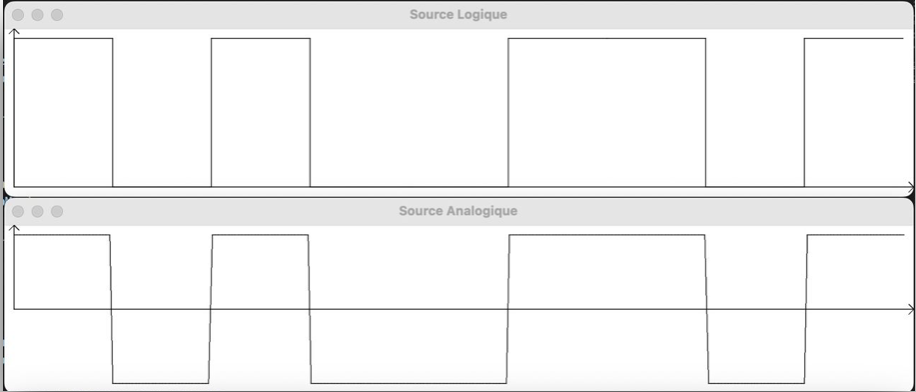
\includegraphics[width=0.5\textwidth]{img/etape2_transmission_NRZ.png}
    \caption{Transmission NRZ}
    \label{fig:teb1}
\end{figure}

On observe bien au niveau de la source analogique que pour un bit un 1 en entrée on a une amplitude d’une valeur de 1. Alors que pour une bit à 0 en entrée, on a une amplitude de -1. La figure ci-dessus illustre bien la conversion du signal logique en signal analogique, étant donnée que l’amplitude pour les 0 logiques n’est plus de 0 mais bien de -1.

\subsubsection{Émission analogique NRZT}

Le codage NRZT (NRZ Trapézoïdal) reprend le même principe que le codage NRZ. C’est à dire que l’on réalise la transmission d’un signal via un système d’échelonnage, avec deux états binaires simple et aucun  niveau intermédiaire. Ce qui diffère est le temps de montée et descente entre deux états binaires, ce qui a pour conséquence  de faire apparaître une pente au début et à la fin du bit. Du fait de ce nouveau facteur, on aura un codage différent selon selon la valeur des symboles précédents et suivants.

\begin{figure}[H]
    \centering
    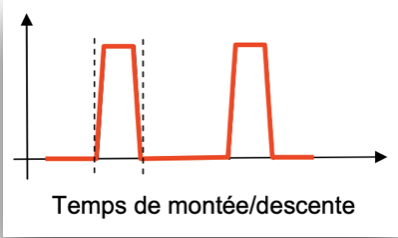
\includegraphics[width=0.33\textwidth]{img/etape2_temps_NRZT.png}
    \caption{Temps bit NRZT}
    \label{fig:teb1}
\end{figure}

D’après ce que l’on a dit précédemment, on peut en déduire que l’on va devoir utiliser des nombres flottant pour pouvoir coder la montée/descente. Cela va impacter la manière dont on code les symboles, chaque symbole pouvant être découper en 3 temps :

\begin{itemize}
    \item Le premier temps : le temps de montée du symbole (1/3 de la période)
    \item Le deuxième temps : l’amplitude Amax/Amin est atteint (1/3 de la période)
    \item Le troisième temps : le temps de la descente du symbole (1/3 de la période)
\end{itemize}

Si on rencontre le cas où il y a deux bits logiques successives de même valeur, il n’y a pas descente. La descente aura lieu au moment où la valeur du bit logique changera.

\begin{figure}[H]
    \centering
    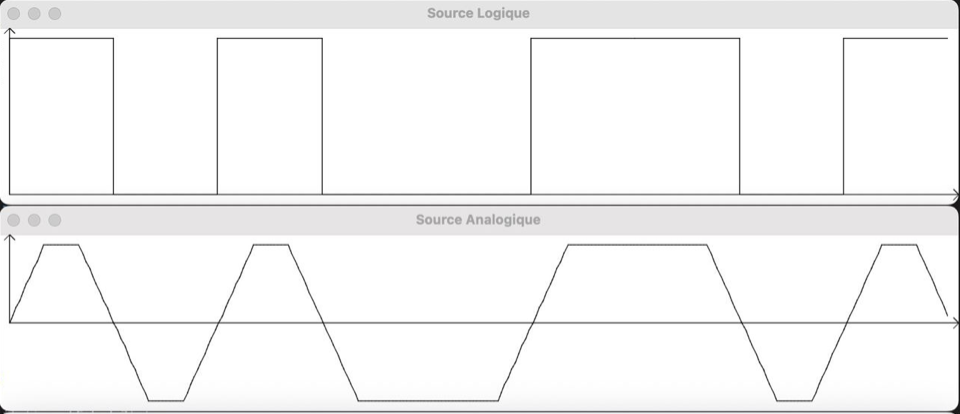
\includegraphics[width=0.5\textwidth]{img/etape2_emission_NRZT.png}
    \caption{Émission NRZT}
    \label{fig:teb1}
\end{figure}

\subsubsection{Émission analogique RZ}

Le codage RZ (Return Zero), il s’agit aussi d’un codage à 2 niveaux. La différence entre NRZ et RZ est que dans le cas du RZ le signal retourne à la valeur 0 entre chaque bit logique codé, même dans le cas de bit logique de même valeur.

\begin{figure}[H]
    \centering
    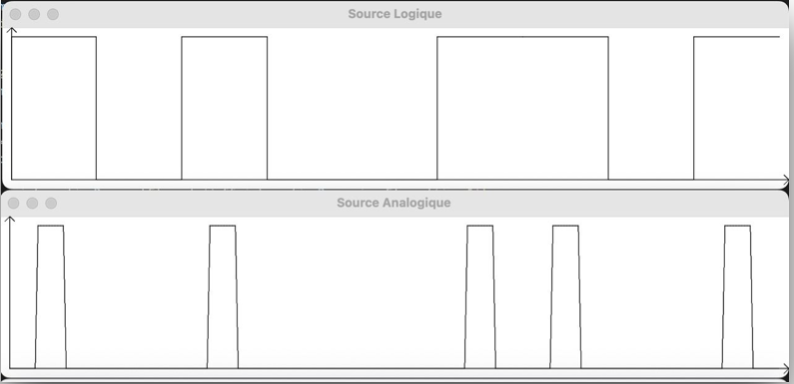
\includegraphics[width=0.5\textwidth]{img/etape2_emission_RZ.png}
    \caption{Émission RZ}
    \label{fig:teb1}
\end{figure}

\subsection{Récepteur analogique}

Nous allons à présent aborder la réception au sein de notre chaîne de transmission. Pour ce faire, nous devons prendre en charge les différentes méthodes de transmission que nous avons précédemment codées, à savoir :

\begin{itemize}
    \item Le NRZ (Non-Return-to-Zero)
    \item Le NRZT (Non-Return-to-Zero with Trailing Zeros)
    \item Le RZ (Return-to-Zero)
\end{itemize}

Une fois que le type de récepteur a été sélectionné, il nous faudra prendre en compte le nombre d'échantillons établis par l'émetteur. Le récepteur reçoit des données au format float et, en fonction du nombre d'échantillons précédemment choisi, il capturera la valeur et appliquera un traitement pour obtenir le codage souhaité.

La classe \textbf{Récepteur} est responsable de la gestion de la réception analogique et prend en charge les trois types de codage mentionnés (NRZ, NRZT et RZ) à travers trois méthodes distinctes, chacune traitant une forme d'onde spécifique.

\subsubsection{Réception analogique NRZ}

La réception d'un signal de type NRZ (Non-Return-to-Zero) repose sur la détection des fronts montants. Dans ce type de signal, les niveaux sont significatifs, et il n'y a pas de niveaux intermédiaires. Pour déterminer la valeur logique de ce signal, on calcule la valeur moyenne du signal analogique NRZ, qui est définie comme la moyenne entre les niveaux maximal ($A_{max}$) et minimal ($A_{min}$) du signal.

Si la valeur lue du signal analogique NRZ est supérieure à la valeur moyenne, alors on interprète cette partie du signal comme étant un 1 logique. Dans le cas contraire, lorsque la valeur est inférieure à la valeur moyenne, on la considère comme étant un 0 logique.

La figure suivante représente le signal analogique NRZ en haut et sa version logique correspondante en bas, illustrant ainsi le processus décris. Le message représenté est \texttt{101001101}.

\begin{figure}[H]
    \centering
    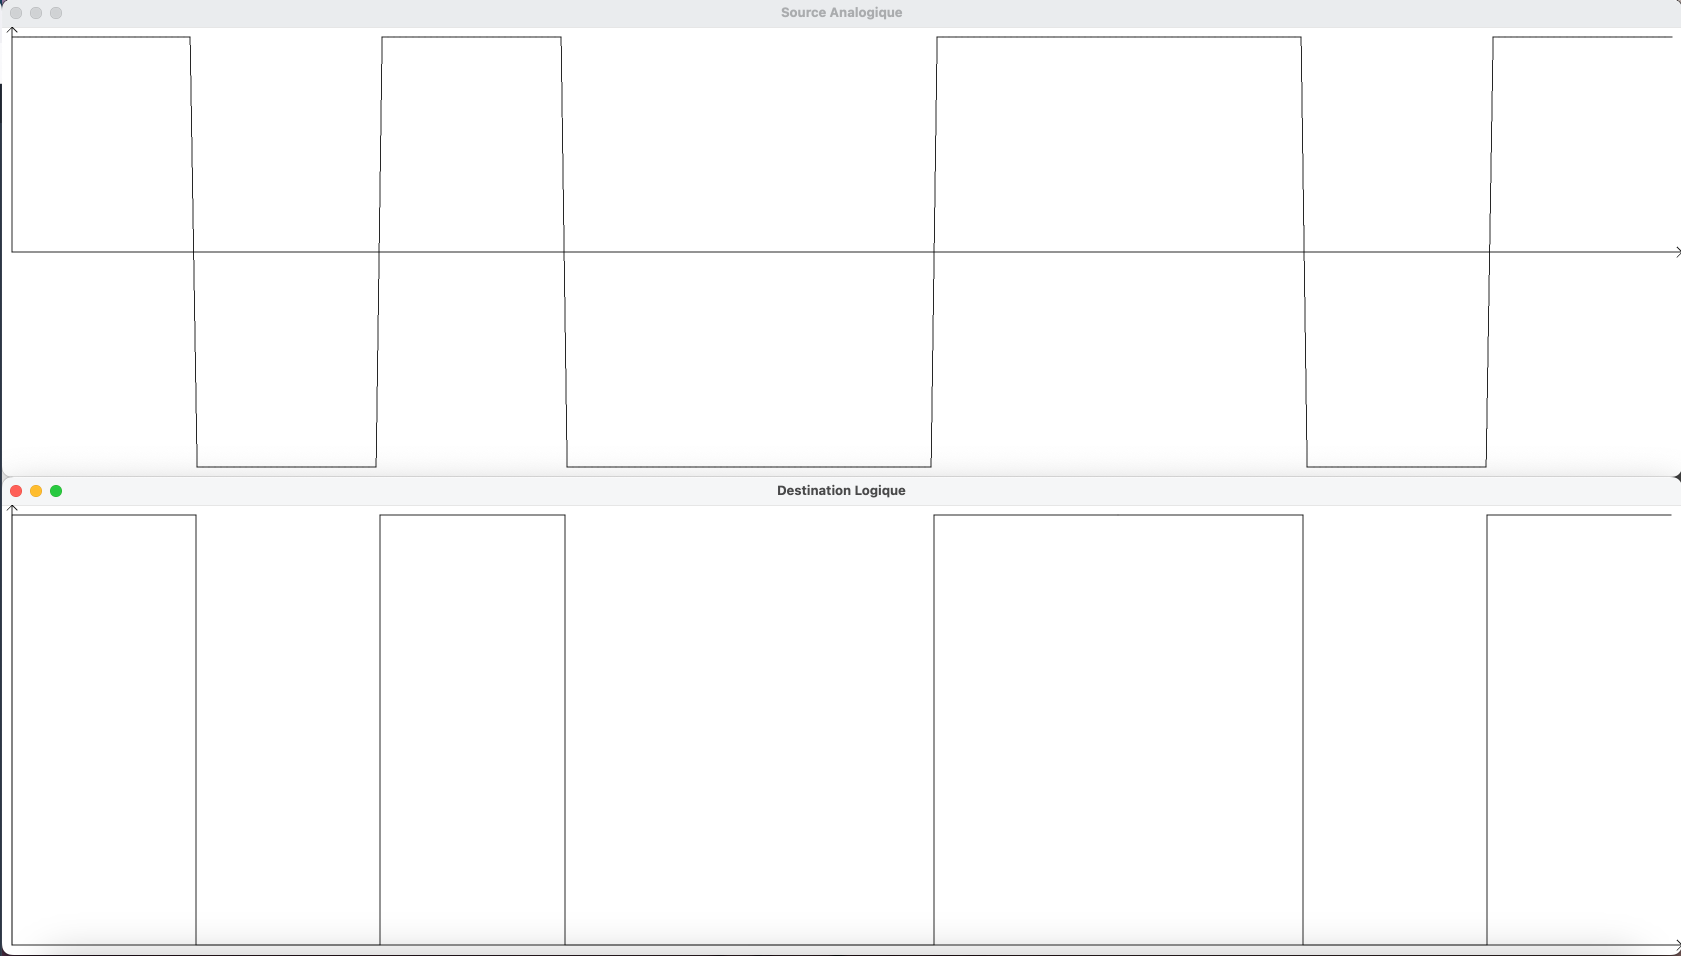
\includegraphics[width=0.5\textwidth]{img/etape2_reception_NRZ.png}
    \caption{Réception NRZ}
    \label{fig:teb1}
\end{figure}

\subsubsection{Réception analogique NRZT}

La réception d'un signal de type NRZT (Non-Return-to-Zero with Trailing Zeros) repose sur la détection de seuil, une technique spécifique qui améliore la fiabilité de la réception des données. Pour ce faire, un indice est positionné au milieu de la durée d'émission d'un bit, ce qui permet une évaluation précise de sa valeur. Cette approche est particulièrement utile pour les signaux NRZT, car elle permet de distinguer efficacement entre les valeurs 0 et 1.

Lorsque l'indice de milieu de bit est atteint, une mesure est effectuée, et la valeur résultante est comparée à un seuil prédéfini. Si la valeur mesurée est supérieure à zéro, le bit mesuré est considéré comme étant 1. En revanche, si la valeur mesurée est inférieure ou égale à zéro, le bit est fixé à 0. Cette méthode de détection de seuil permet de minimiser les erreurs de décodage, car elle tient compte de la valeur relative par rapport à un point de référence au milieu du bit.

La figure ci-dessous illustre le processus de transmission de données utilisant le codage NRZT (Non-Return-to-Zero with Trailing Zeros). En haut, vous pouvez voir un signal analogique généré par la source,  et en bas, le signal logique reçu par la destination est représenté. Le message envoyé est \texttt{101001101}. Cette représentation visuelle montre comment le signal analogique est encodé et décodé pour obtenir la séquence de bits d'origine. 

\begin{figure}[H]
    \centering
    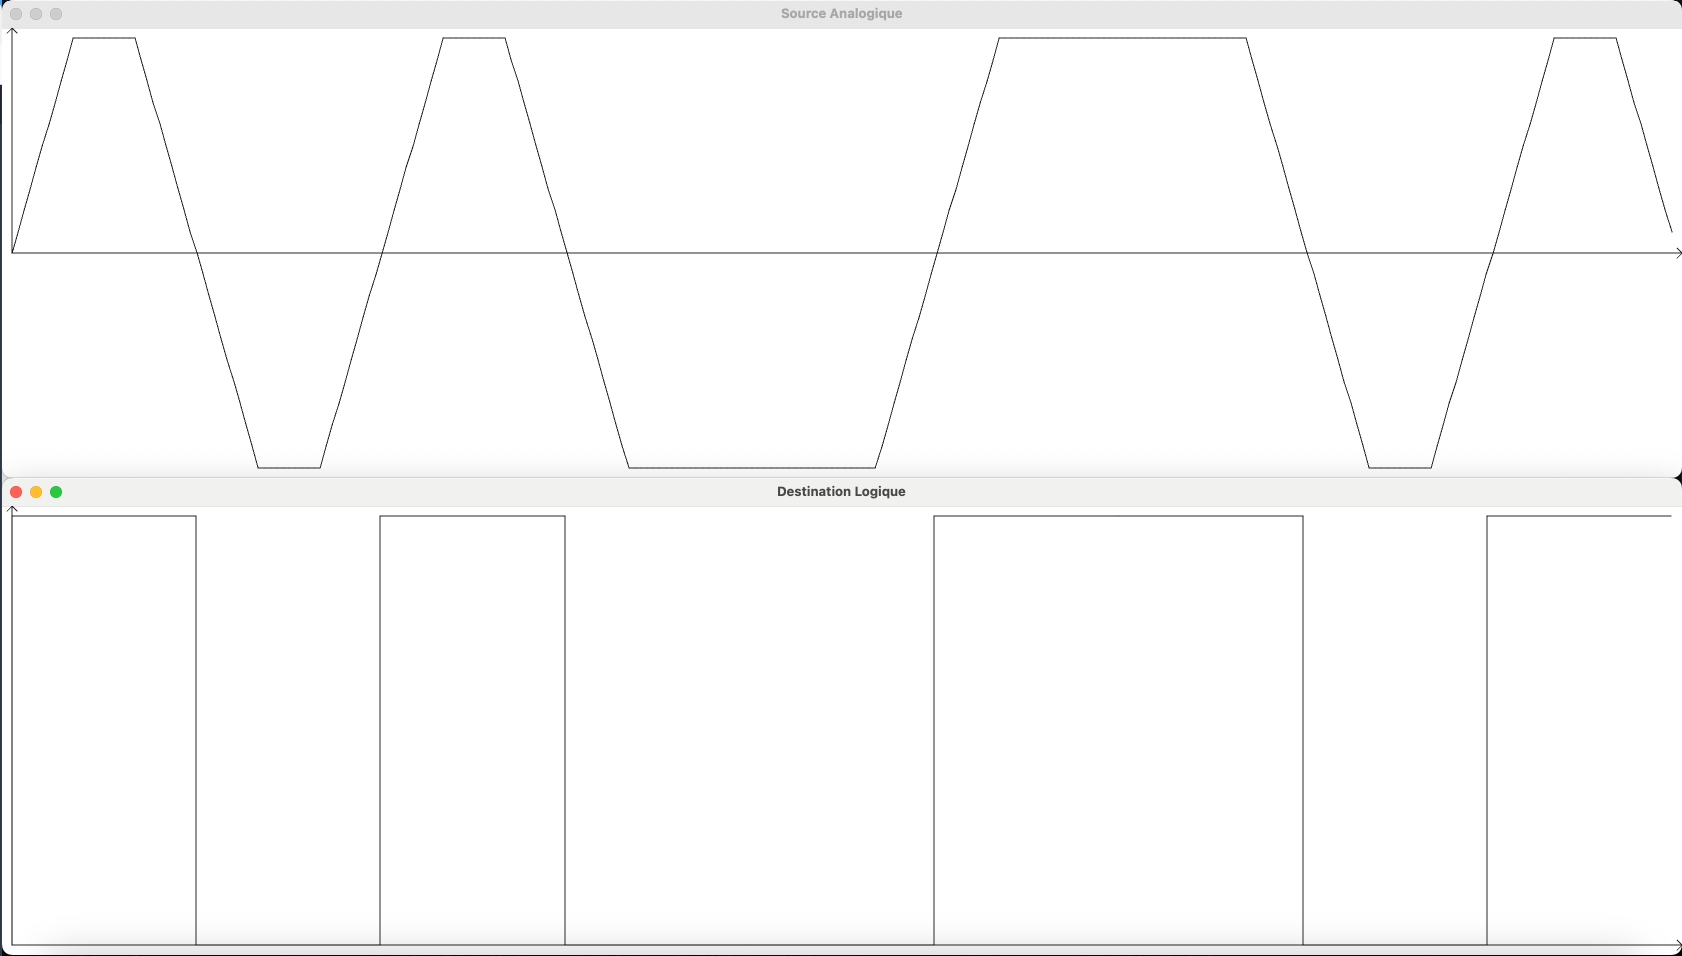
\includegraphics[width=0.5\textwidth]{img/etape2_reception_NRZT.png}
    \caption{Réception NRZT}
    \label{fig:teb1}
\end{figure}

\subsubsection{Réception analogique RZ}

Le codage RZ (Return-to-Zero) présente la particularité de revenir à zéro à chaque période de bit. Cela se traduit par la présence de deux transitions potentielles par période, généralement au milieu de celle-ci. Lorsqu'un 1 est transmis, le signal atteint son pic au milieu de la période et retourne ensuite à zéro. En revanche, lorsqu'un 0 est envoyé, le signal reste à zéro.

Le décodage du RZ repose sur la détection de ces transitions, notamment celles qui se produisent au milieu de chaque période de bit. Une transition détectée est interprétée comme un 1, tandis qu'aucune transition équivaut à un 0. 

La figure ci-dessous illustre la source analogique RZ en haut et le signal logique reçu par la destination en bas. Le message transmis correspond à la séquence binaire \texttt{101001101}.

\begin{figure}[H]
    \centering
    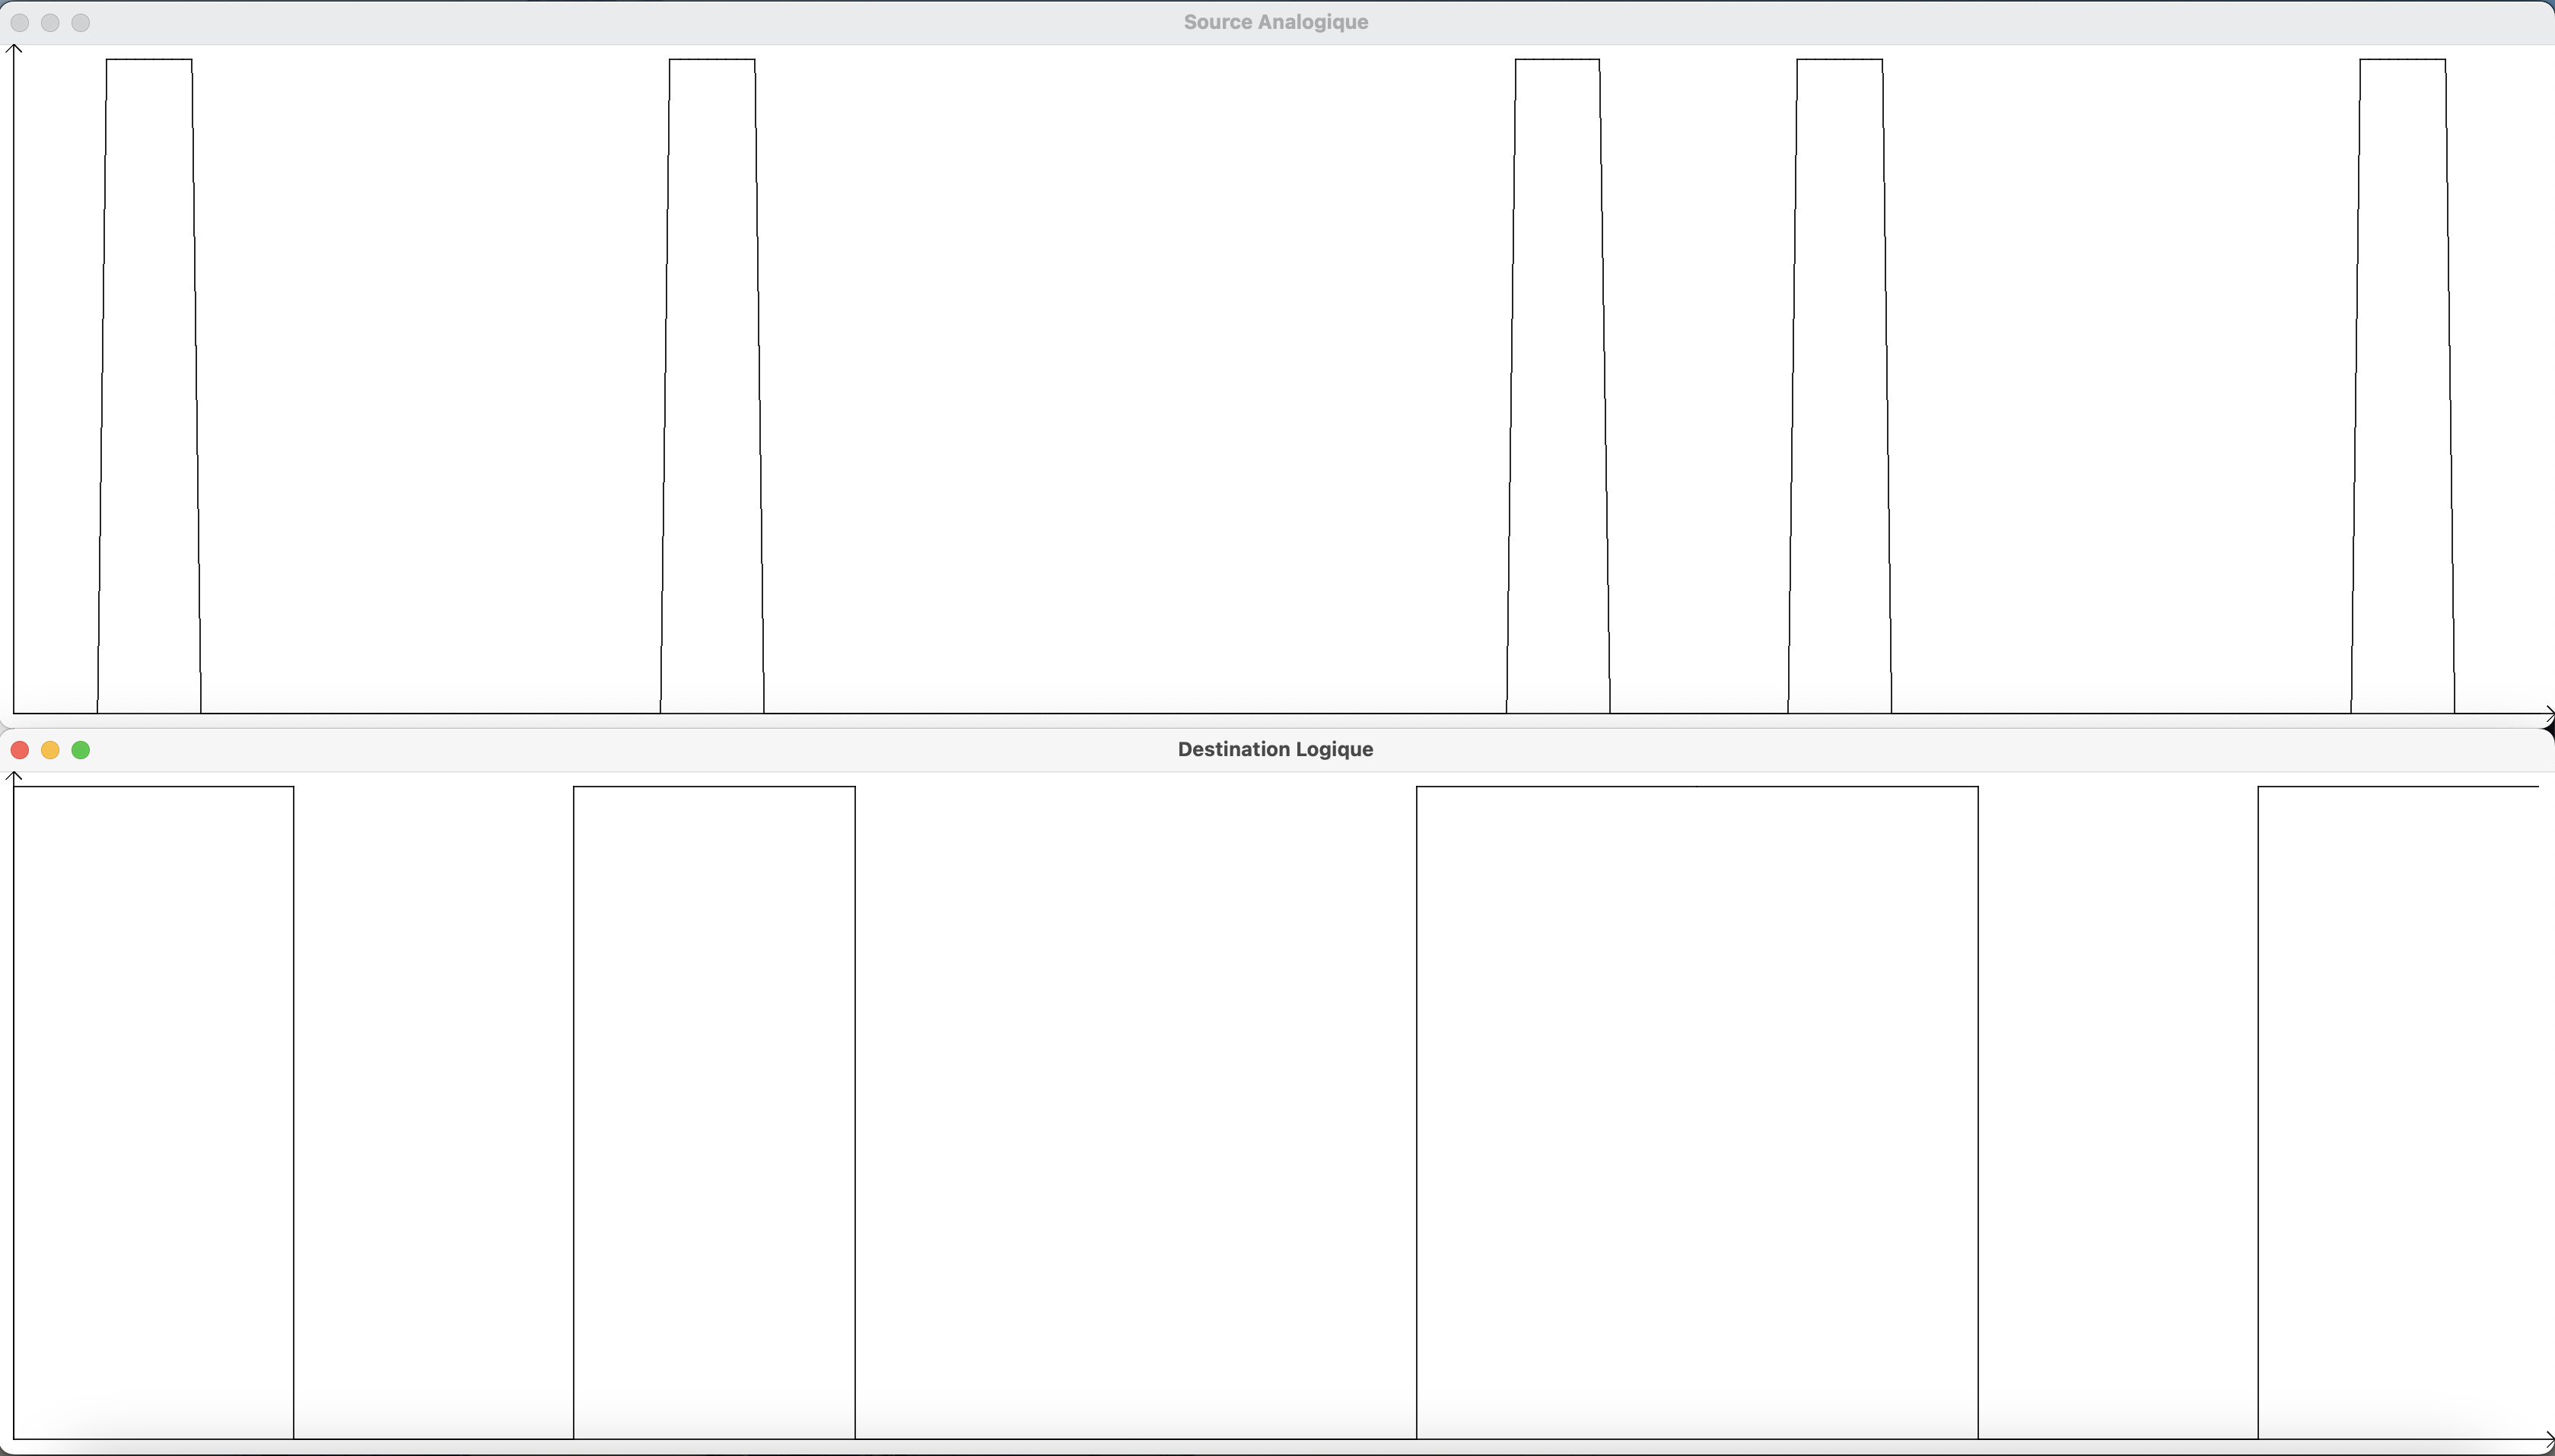
\includegraphics[width=0.5\textwidth]{img/etape2_reception_RZ.png}
    \caption{Réception RZ}
    \label{fig:teb1}
\end{figure}

\subsubsection{Conclusion étape 2}

L'étape 2 de notre projet de transmission a permis la mise en œuvre de différentes méthodes de codage, à savoir NRZ, NRZT et RZ. Contrairement à l'étape précédente, où seule une transmission logique était en place entre la source et la destination, cette étape a introduit une dimension analogique dans notre chaîne de transmission. 

Nous avons observé comment le codage NRZ maintient des niveaux stables pour les valeurs binaires 0 et 1, tandis que le NRZT utilise la détection de seuil pour distinguer efficacement ces valeurs au moyen de transitions au milieu de chaque bit. Enfin, le codage RZ présente la particularité de revenir à zéro au milieu de chaque période de bit (à 1), améliorant ainsi la synchronisation entre l'émetteur et le récepteur.

Il est important de noter que, pour le moment, nous n'avons pas pris en compte la présence de bruit dans notre système, ce qui signifie que le TEB (Taux d'Erreur Binaire) est de 0\%, garantissant une transmission parfaitement fiable. 